\lecture[4]{4. Föll af mörgum breytistærðum}{lecture-text}
\date{14.~janúar 2015}
\newcounter{mycount}
\refstepcounter{mycount}

\begin{document}

\begin{frame}
	\maketitle
\end{frame}




\begin{frame}{Graf falls} 

\begin {block}{Skilgreining 4.\arabic{mycount}}\stepcounter{mycount}
Látum $f:\R^2\rightarrow \R$ vera fall.  {\em Graf} fallsins er skilgreint sem mengið 
$$\{(x,y,f(x,y))\mid (x,y)\in\R^2\}\subseteq \R^3.$$

Ef $f:\R^3\rightarrow \R$ er fall, þá er  {\em graf} fallsins skilgreint sem mengið 
$$\{(x,y,z,f(x,y,z))\mid (x,y,z)\in\R^3\}\subseteq \R^4.$$
\end{block}
            
\end{frame}

\begin {frame}{Graf falls}
 Dæmi: $f(x,y) = \sqrt{1-x^2-y^2}$, $-0.5\leq x,y\leq 0.5$.         

\begin{figure} [h]
\begin {center} \scalebox{0.45 }{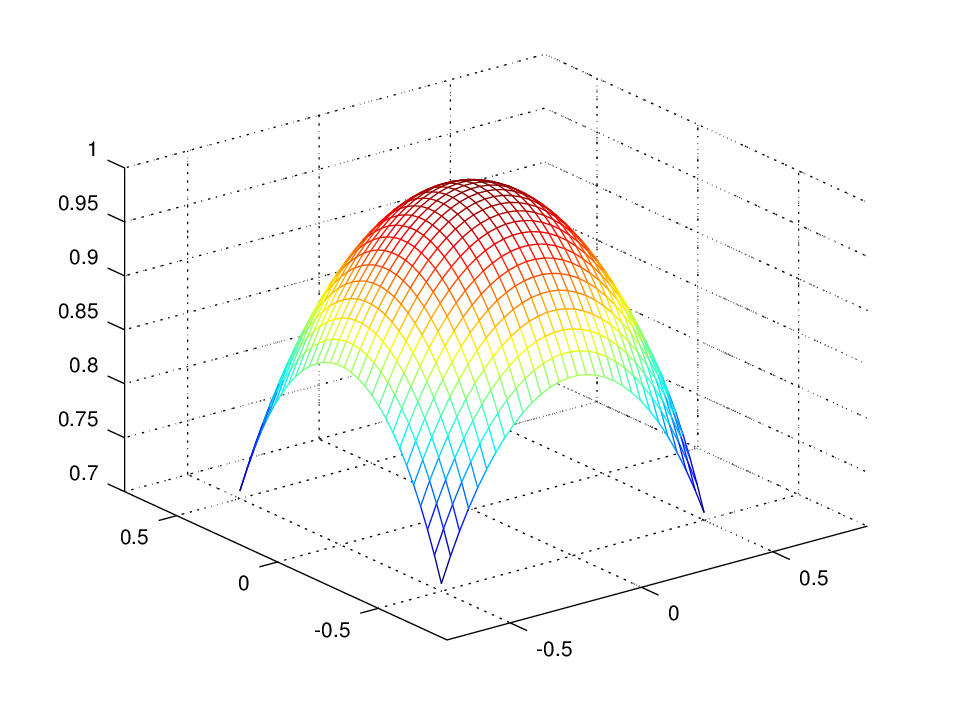
\includegraphics{surface.png}} \end {center}
\end {figure}  
\end {frame}


\begin {frame}{Jafnhæðarlínur}
 \begin {block} {Skilgreining 4.\arabic{mycount}}\stepcounter{mycount}
  Látum $f:\R^2\rightarrow \R$ vera fall.  Ef $c$ er fasti þá er mengið 
$$\{(x,y)\mid f(x,y)=c\}\subseteq \R^2$$
kallað {\em jafnhæðarlína} eða {\em jafnhæðarferill} (e.~level curve) fallsins $f$ fyrir fastann $c$.

 Látum $f:\R^3\rightarrow \R$ vera fall.  Ef $c$ er fasti þá er mengið 
$$\{(x,y,z)\mid f(x,y,z)=c\}$$
kallað {\em jafnhæðarflötur} (e.~level surface)  
fallsins $f$ fyrir fastann $c$.
 \end {block}
\end {frame}

\begin {frame}{Jafnhæðarlínur}
 Dæmi: $f(x,y) = \sqrt{1-x^2-y^2}$, $-0.5\leq x,y\leq 0.5$.         

\begin{figure} [h]
\begin {center} \scalebox{0.45 }{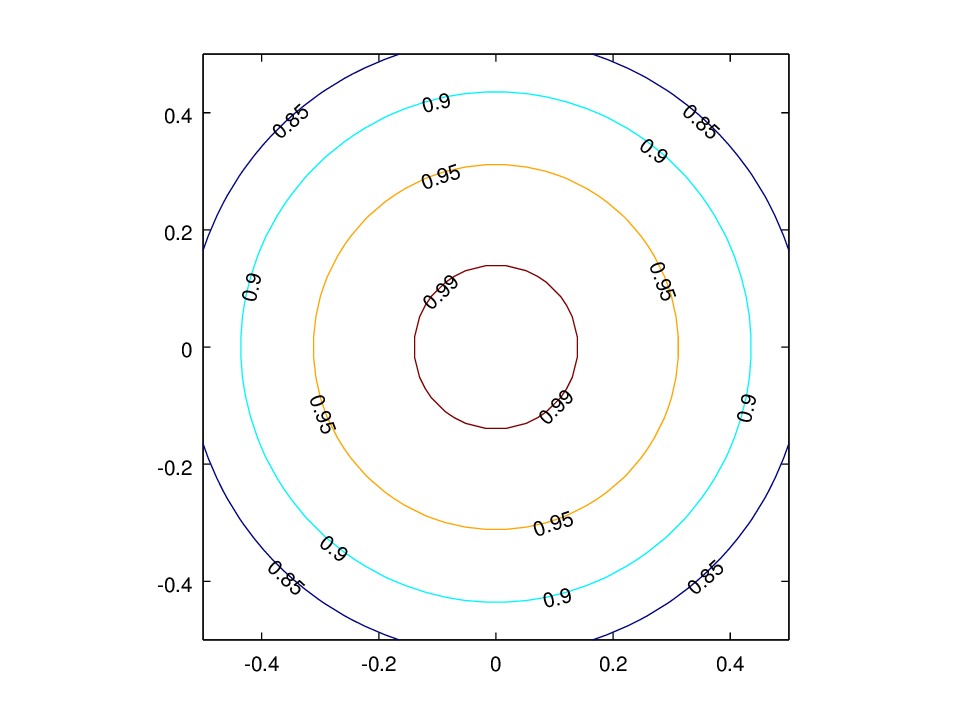
\includegraphics{contour.png}} \end {center}
\end {figure}  
\end {frame}

\begin {frame}{Fjarlægð milli punkta}
\begin {block}{Skilgreining 4.\arabic{mycount}}\stepcounter{mycount}
 {\em Fjarlægðin} milli tveggja punkta 
$\xv=(x_1,x_2, \ldots,x_n)$ og $\yv=(y_1,y_2, \ldots,y_n)$ í $\Rn$ er skilgreind sem talan
$$|\xv-\yv|=\sqrt{(x_1-y_1)^2+(x_2-y_2)^2+\cdots+(x_n-y_n)^2}.$$
 \end {block}

\end {frame}

\begin {frame}{Opnar kúlur}
 \begin {block}{Skilgreining 4.\arabic{mycount}}\stepcounter{mycount}
  Látum $P=(p_1,p_2,\ldots,p_n)$ vera punkt í
$\Rn$.  Skilgreinum {\em opnu kúluna} með miðju í $P$ og geisla $r$ sem
mengið  
$$B_r(P)=\{Q\in\Rn\mid |Q-P|<r\}.$$
Í $\R^2$ er eðlilegra að tala um {\em opna skífu} eða {\em opinn disk} í stað opinnar kúlu og í $\R$ þá er talað um opin bil.  

 \end {block}

\end {frame}


\begin {frame}{Opin mengi}
 \begin {block}{Skilgreining 4.\arabic{mycount}}\stepcounter{mycount}
Látum $U$ vera hlutmengi í $\Rn$.

Sagt er að $U$ sé {\em opið mengi} ef um sérhvern punkt $P$ í $U$ gildir að til er tala $r>0$ þannig að $B_r(P)\subseteq U$.

Mengið $U$ er sagt {\em lokað} ef fyllimengið er opið.  ({\em Fyllimengi} $U$ er skilgreint sem mengið 
$\Rn\setminus U=\{Q\in \Rn\mid Q\nin U\}$.)
\end {block}

\end {frame}

\begin {frame}{Jaðarpunktur}
 \begin {block}{Skilgreining 4.\arabic{mycount}}\stepcounter{mycount}
Látum $U$ vera mengi í $\Rn$.  Punktur $P$ í $\Rn$ er sagður {\em jaðarpunktur} $U$ ef sérhver opin kúla $B_r(P)$ með $r>0$ inniheldur bæði punkt úr $U$ og punkt úr $\Rn\setminus U$.   (Athugið að bæði er mögulegt að jaðarpunktur $U$ sé í $U$ og að hann sé ekki í $U$.)
\end {block}
\end {frame}

\begin {frame}{Skilgreiningarmengi}
 \begin {block}{Skilgreining 4.\arabic{mycount}}\stepcounter{mycount}
Fyrir fall $f(x_1,x_2,\ldots,x_n)$ þá táknar ${\cal D}(f)$ skilgreiningarmengi fallsins $f$.
Ef fallið er gefið með formúlu og ekkert sagt um ${\cal D}(f)$ þá lítum við svo á að ${\cal D}(f)$ sé mengi allra punkta í $\Rn$ þannig að formúlan gefi vel skilgreinda tölu.
\end {block}
\end {frame}


\begin {frame}{Markgildi}
 \begin {block}{Skilgreining 4.\arabic{mycount}}\stepcounter{mycount}
Látum $f(x_1,x_2,\ldots,x_n)$ vera fall af
$n$ breytistærðum með skilgreiningarmengi ${\cal D}(f)\subseteq \Rn$.
Látum $P=(p_1,p_2,\ldots,p_n)$ vera punkt í $\Rn$ þannig að sérhver
opin kúla um $P$ inniheldur meira en einn punkt úr ${\cal D}(f)$. 

\smallskip 
\noindent
Segjum að $f(x_1,x_2,\ldots,x_n)$  stefni á tölu $L$ þegar
$(x_1,x_2,\ldots,x_n)$  stefnir á $(p_1,p_2,\ldots,p_n)$ ef
eftirfarandi gildir: 

\smallskip
\noindent
{\em Fyrir sérhverja tölu $\epsilon>0$ er til tala $\delta>0$
þannig að ef $(x_1,x_2,\ldots,x_n)\in{\cal D}(f)$ og  
$$|(x_1,x_2,\ldots,x_n)-(p_1,p_2,\ldots,p_n)|<\delta$$ 
þá er 
$$|f(x_1,x_2,\ldots,x_n)-L|<\epsilon.$$}
\end{block}
\end {frame}

\begin {frame}{Markgildi}
\begin {block}{Ritháttur 4.\arabic{mycount}}\stepcounter{mycount}
Ef $f(x_1,x_2,\ldots,x_n)$  stefnir á tölu $L$ þegar $(x_1,x_2,\ldots,x_n)$  stefnir á $(p_1,p_2,\ldots,p_n)$ þá er ritað 
$$\lim_{(x_1,x_2,\ldots,x_n)\rightarrow (p_1,p_2,\ldots,p_n)}
f(x_1,x_2,\ldots,x_n)=L.$$
 \end {block}
\end {frame}

\begin {frame}{Markgildi}
 \begin {block}{Skilgreining 4.\arabic{mycount} (Skilgreining 4.8 sett fram fyrir föll af tveimur breytum.)  }\stepcounter{mycount}
 
  
Látum $f(x,y)$ vera fall skilgreint á mengi  ${\cal D}(f)\subseteq \R^2$.  Látum $(a,b)$ vera punkt í $\R^2$ þannig að sérhver opin skífa um $(a,b)$ inniheldur meira en einn punkt úr ${\cal D}(f)$.

Segjum að $f(x,y)$  stefni á tölu $L$ þegar $(x,y)$  stefnir á $(a,b)$ ef eftirfarandi gildir:

\smallskip
\noindent
{\em fyrir sérhverja tölu $\epsilon>0$ er til tala $\delta>0$
þannig að ef $(x,y)\in{\cal D}(f)$ og
$$\delta>|(x,y)-(a,b)|=\sqrt{(x-a)^2+(y-b)^2}$$ 
þá er  
$$|f(x,y)-L|<\epsilon.$$}

 \end {block}

\end {frame}


\begin {frame}{Reglur um markgildi}
 \begin {block}{Setning 4.\arabic{mycount}}\stepcounter{mycount}
  Látum $f$ og $g$ vera föll af tveimur breytum.  Gerum ráð  fyrir að 
$$\lim_{(x,y)\rightarrow (a,b)}f(x,y)=L\quad\mbox{og}\quad
\lim_{(x,y)\rightarrow (a,b)}g(x,y)=M,$$
og að sérhver grennd um $(a,b)$ innihaldi fleiri en einn punkt þar sem bæði föllin $f$ og $g$ eru skilgreind. Þá gildir

{\bf (a)}  $\lim_{(x,y)\rightarrow (a,b)}(f(x,y)\pm g(x,y))=L\pm M$.

{\bf (b)}  $\lim_{(x,y)\rightarrow (a,b)}f(x,y) g(x,y)=LM$.

{\bf (c)}  $\lim_{(x,y)\rightarrow (a,b)}\frac{f(x,y)}{g(x,y)}=
\frac{L}{M}$, svo framarlega sem $M\neq 0$.

{\bf (d)}  $\lim_{(x,y)\rightarrow (a,b)}F(f(x,y))=F(L)$ ef $F$ er fall af einni breytistærð sem er samfellt í punktinum $L$.
 
 \end {block}

\end {frame}


\begin {frame}{Samfelldni}
 \begin {block}{Skilgreining 4.\arabic{mycount}}\stepcounter{mycount}
   Látum $f$ vera fall af $n$ breytistærðum skilgreint á mengi ${\cal D}(f)$ í $\Rn$.  Fallið $f$ er sagt {\em samfellt í punkti} $ (p_1,p_2,\ldots,p_n)$ í ${\cal D}(f)$  ef 
$$\lim_{(x_1,x_2,\ldots,x_n)\rightarrow (p_1,p_2,\ldots,p_n)}
f(x_1,x_2,\ldots,x_n)=f(p_1,p_2,\ldots,p_n).$$

Sagt er að fallið sé {\em samfellt} ef það er samfellt í öllum punktum skilgreiningarmengis síns.

 \end {block}

\end {frame}




\end{document}